
\section{Design}
\begin{figure*}
\centering
\begin{subfigure}{0.41\linewidth}
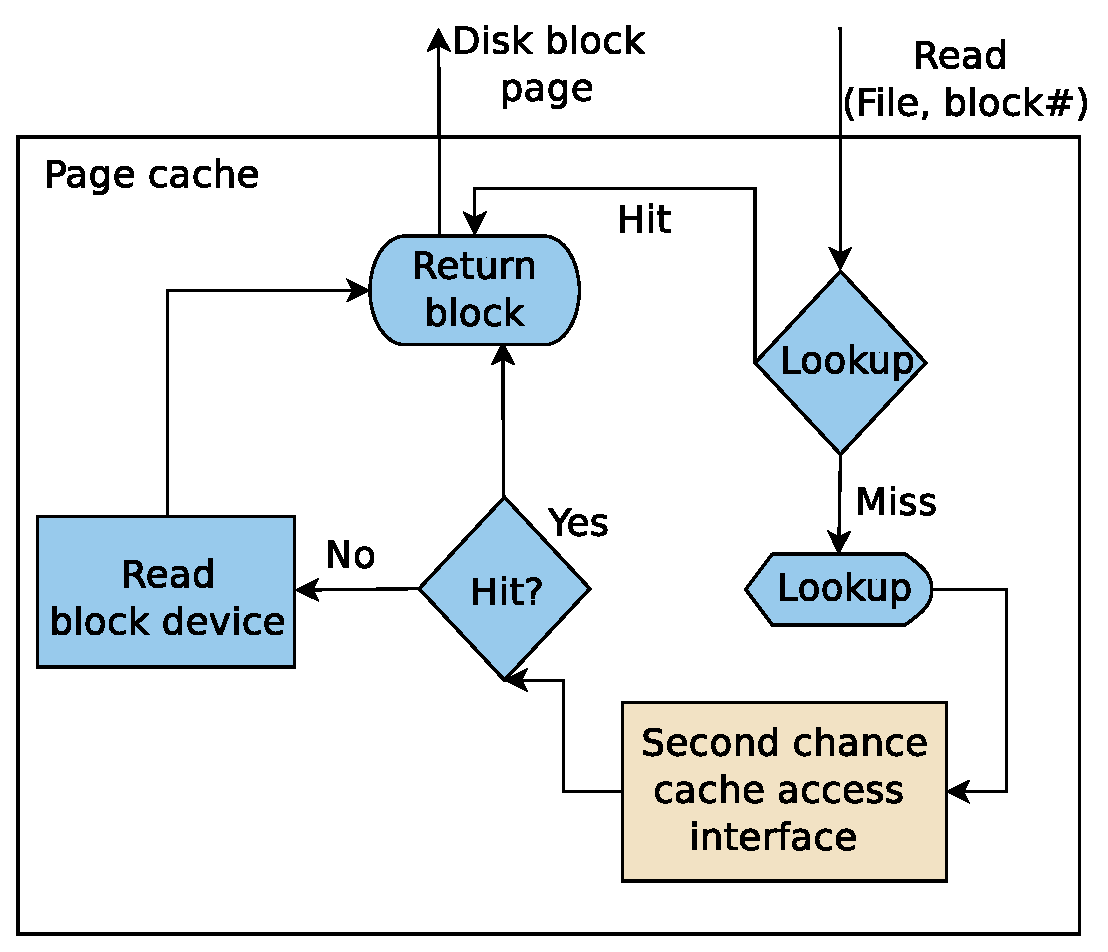
\includegraphics[width=\columnwidth]{images/cc_get}
 \caption{I am part-1}
 \label{fig:part1}
\end{subfigure} \hfill
%
\begin{subfigure}{0.41\linewidth}
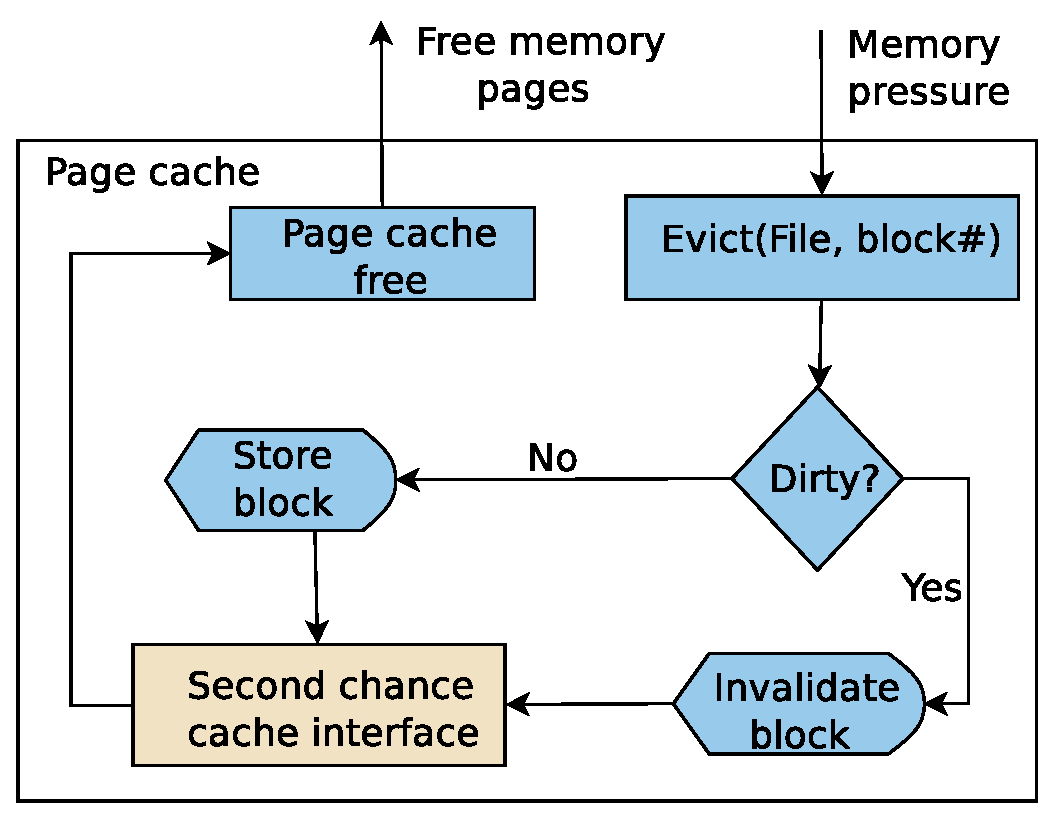
\includegraphics[width=\columnwidth]{images/evict}
 \caption{I am part-2}
 \label{fig:part2}
\end{subfigure} \hfill
%
\caption{This is a composite figure containing two sub-figures.}
\label{fig:composite}
\end{figure*}

An example to write algorithms follow.
\subsection{Insertion sort algorithm}

\begin{algorithm}
  \caption{Another way to write insertion sort}
  \label{algo:ins_sort1}
  \begin{algorithmic}[1]
     \Procedure{InsertionSort}{A[0..N]}\newline
     \Comment{A is an array of N integers}
      \State $i \leftarrow$ 1
      \While {($i <  N$)}
          \State $j \leftarrow i$ \newline
           \Comment{Iterate to find the place for this element in the sorted array}
         \While {($j > 0$ and $A[j-1] > A[j]$)}
            \State \textit{swap}($A[j]$, $A[j-1]$)
            \State $j \leftarrow j -1$ 
         \EndWhile
      \State $i \leftarrow i + 1$
      \EndWhile
     \EndProcedure 
  \end{algorithmic}
\end{algorithm}



\lipsum[50]

\lipsum[50]

As shown in Figure~\ref{fig:composite}, there are two subcomponents---Part(1) in Figure~\ref{fig:part1}
and Part(2) in Figure~\ref{fig:part2}.


\begin{table}[t]
\scriptsize
\begin{center}
\begin{tabular}{|c|c|c|c|}
\hline
{\bf Assign-} & {\bf Topic} & {\bf \#of} & {\bf Avg.} \\
{\bf -ment} & & {\bf submissions} & {\bf marks (/30)} \\
\hline
\hline
I & Bash & 90 & 20 \\
%\hline
II & AWK &  80 & 18.5 \\
%\hline
III & Python & 100 & 24 \\
%\hline
IV & Latex & 110 & 29 \\
\hline
\end{tabular}
\caption{This is a simple table showing assignment submission statistics.}
\label{table:simple}
\end{center}
\end{table}

Table~\ref{table:simple} shows phony data regarding CS251 assignment submission.
\lipsum[50]

\subsection{Equations and Symbols}
Some basic trigonometric identities are as follows,
\begin{equation}
\sin^2\theta + \cos^2\theta = 1
\end{equation}

\begin{equation*}
\sin(\alpha + \theta) = \sin \alpha \cos \theta + \cos \alpha \sin \theta
\end{equation*}

\indent
\begin{align}
\sin(\frac{\pi}{2} -\theta) &= \cos\theta \\
1 + \tan^2 \theta &= \sec^2 \theta\\
1 + \cot^2 \theta &= \csc^2 \theta
\end{align}

Now let us write some equations from calculus.
\begin{equation*}
\lim_{x \to \infty} \frac{\sin x}{x} = 1
\end{equation*}

\begin{align*}
\sum_{i=1}^n i^2 &= \frac{1}{2} n (n+1) \\
\int_0^{\frac{\pi}{2}} \cos\theta\,d\theta &= \sin\theta\Big|_0^\frac{\pi}{2} \\
  &= \sin\frac{\pi}{2} - \sin 0 \\
  &= 1 \\
\end{align*}
If  $f(x) = x^2 + 2x + 1$, \\ 
Then  $\frac{df(x)}{dx} = 2x + 2$ 

